\chapter{参考文献について}
\section{引用順にソート済みであることの確認}
例えば,「$1935$年にA.~Einsteinらは後に量子論が不完全と主張した~\cite{PhysRev.47.777}が,
彼らの主張では実験的に検証可能でなかった.
しかし,約$30$年の月日が経った$1964$年にJ.~S.~BellがA.~Einsteinらの主張が検証可能であることを示した~\cite{PhysicsPhysiqueFizika.1.195}.」と書いて引用するとき,自動で引用順になる.

引用順になる理由は,
main\_LuaTeX.texでのbiblatexパッケージの公式ドキュメント~\cite{biblatex}を参照すること.

% === figure === %
\begin{figure}[h]
  \centering
  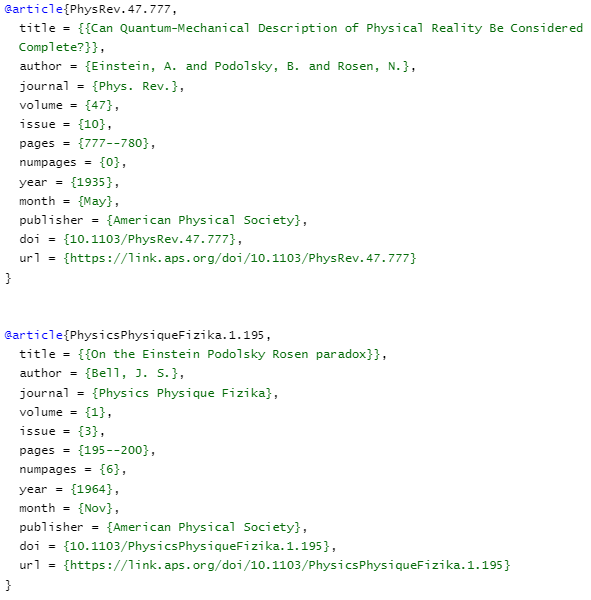
\includegraphics[keepaspectratio, width=0.6\linewidth]{ref_series.png}
  \caption{reference.bibの中にある参考文献の順番を表している図である.
  ``PhysicsPhysiqueFizika.1.195''が``PhysRev.47.777''よりも先に書かれているが,
  引用順は反対なため出力されたこのPDF内での参考文献の順番は反対になっている.
  したがって,参考文献をreferences.bibに載せる順番はまったく気にしなくてもよいことがいえる.}
  \label{fig:ref_series}
\end{figure}
% === figure === %

\section{参考文献の設定}
このテンプレートでは,Bib\LaTeX を採用した.
注意点としては,\textcolor{red}{Bib\TeX とは異なる}という点である.
このため,誤ってBib\TeX で検索しないように注意すること.
図\ref{fig:biblatex_settings}にBib\LaTeX の設定を示した.

このテンプレートでは,参考文献をIEEEスタイルで表示するようにしているが,
各指導教官の方々の指示に従い,適宜変更すること.
なお,変更する際は公式ドキュメント~\cite{biblatex}やその他サイトで
検索して調べるように.

% === figure === %
\begin{figure}[h]
  \centering
  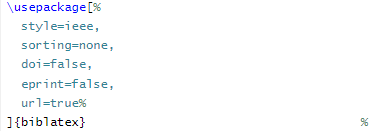
\includegraphics[keepaspectratio, width=0.6\linewidth]{biblatex_settings.png}
  \caption{main\_LuaTeX.texのBib\LaTeX の設定を示している.同ファイルの$16$行目にある.}
  \label{fig:biblatex_settings}
\end{figure}
% === figure === %

\section{Bibファイル編集の注意点}
図\ref{fig:ref_series}を見ると,titleを示す箇所が$2$重波括弧 \{\{\}\} で囲われている.
これは通常の波括弧 \{\} ではBib\LaTeX で先頭のみが大文字になる(有名な?)問題があり,
回避するには$2$重波括弧 \{\{\}\} で囲う必要があるそう.
Bibファイル内のtitleを自動で$2$重波括弧 \{\{\}\} にする方法は調べれば直ぐに出るが,
面倒なので作成していない.
